% vim: set tw=78 sts=2 sw=2 ts=8 aw et ai:
\documentclass[12pt]{article}

\usepackage[paper=a4paper, top=2cm, bottom=3cm, left=2.5cm, right=2.5cm]{geometry}

\usepackage{ucs}
\usepackage[utf8x]{inputenc}
\usepackage[english]{babel}
%\usepackage{hyperref}	  % use \url{http://$URL} or \href{http://$URL}{Name}
\usepackage{underscore}	  % underscores need not be escaped
\usepackage{subfigure}
\usepackage{verbatim}
\usepackage{float}
\usepackage{booktabs}     % professional tables
\usepackage{parskip}

% Support for including graphics
\usepackage{graphicx}
\DeclareGraphicsExtensions{.pdf,.png,.jpg}

\title{A Behavioral Analysis of Multipath TCP}

\author{Silviu Petria, Silviu Popescu\\
Faculty of Automatic Control and Computers\\
University POLITEHNICA of Bucharest\\
Splaiul Independenței 313, Bucharest, Romania, 060042 \\
\emph{\{silviu.petria,silviu.popescu\}@cti.pub.ro}}

\date{\today}

\begin{document}

\maketitle

\begin{abstract}
% vim: set tw=78 sts=2 sw=2 ts=8 aw et ai:
Multipath TCP (MPTCP) is an ongoing effort to extend TCP by allowing a connection to use multiple paths in order to improve resource usage efficiency and offer redundancy. Despite having a working implementation, it still faces obstacles before large scale deployment. This study presents the results of an analysis of MPTCP's behavior in a controlled environment, aiming to understand how parameters such as delay, bandwidth, buffer size and congestion window size affect performance. The final goal of the project is to devise a system that allows users to bypass egress firewalls using MPTCP, OpenVPN and tunneling traffic via common protocols.

\end{abstract}

\section{Introduction}
\label{sec:introduction}
% vim: set tw=78 sts=2 sw=2 ts=8 aw et ai:
Our previous report \cite{sem1} focused on the effect of TCP link configurations over MPTCP. We found that while MPTCP's congestion window algorithm performs very well, the throughput is very much influenced by the size of the receive buffer, which must be correlated with the bandwidth-delay product. We have built on those findings and incorporated them into a new test environment, looking to understand how MPTCP combined throughput is affected when running over OpenVPN tunnels, both UDP and TCP.

OpenVPN is a popular lightweight open source SSL VPN solution that provides a wide range of functionalities including remote access and site-to-site VPNs, together with extensive link security and client authentication capabilities. We have chosen it due to its ubiquity, ease to use and detailed documentation.

\section{Architecture}
\label{sec:architecture}
% vim: set tw=78 sts=2 sw=2 ts=8 aw et ai:

Design and architectural details.


\section{Implementation}
\label{sec:implementation}
% vim: set tw=78 sts=2 sw=2 ts=8 aw et ai:

Proper implementation is proper.


\section{Experimental Setup}
\label{sec:setup}
% vim: set tw=78 sts=2 sw=2 ts=8 aw et ai:

Having previously presented the various aspects that factor into MPTCP
performance, the current section describes how a highly configurable computer
network was modeled. A solution suitable to our analysis should preferably
yield similar results for several runs of a single test, grant the ability to
control the features outlined in \ref{sec:tcp-link} in a fine-grained manner
and also require comodity hardware. To this end, our experiments are based on
Mininet, a framework well suited for software defined networking. Being both
scalable and flexible, it conforms to the criteria mentioned above.

Mininet uses features of lightweight virtualization available on Linux
systems, such as process and network namespaces\cite{mininet}. There is a root
namespace, the default on a Linux system, which houses the switches, the
controller and the main management application. There is another distinct
namespace for each host, providing a network interface and a shell. The hosts'
interfaces are paired with counterparts in the root namespace and the shells
are piped to the management console, as can be observed in Figure
\ref{fig:mininet-design}. By using this approach, the overhead associated with
adding a new node to the simulation is negligible. Additionally, the framework
supports Open vSwitch, a virtual switch implemented in the kernel, for
modelling basic network equipment.

\begin{figure}
  \centering
  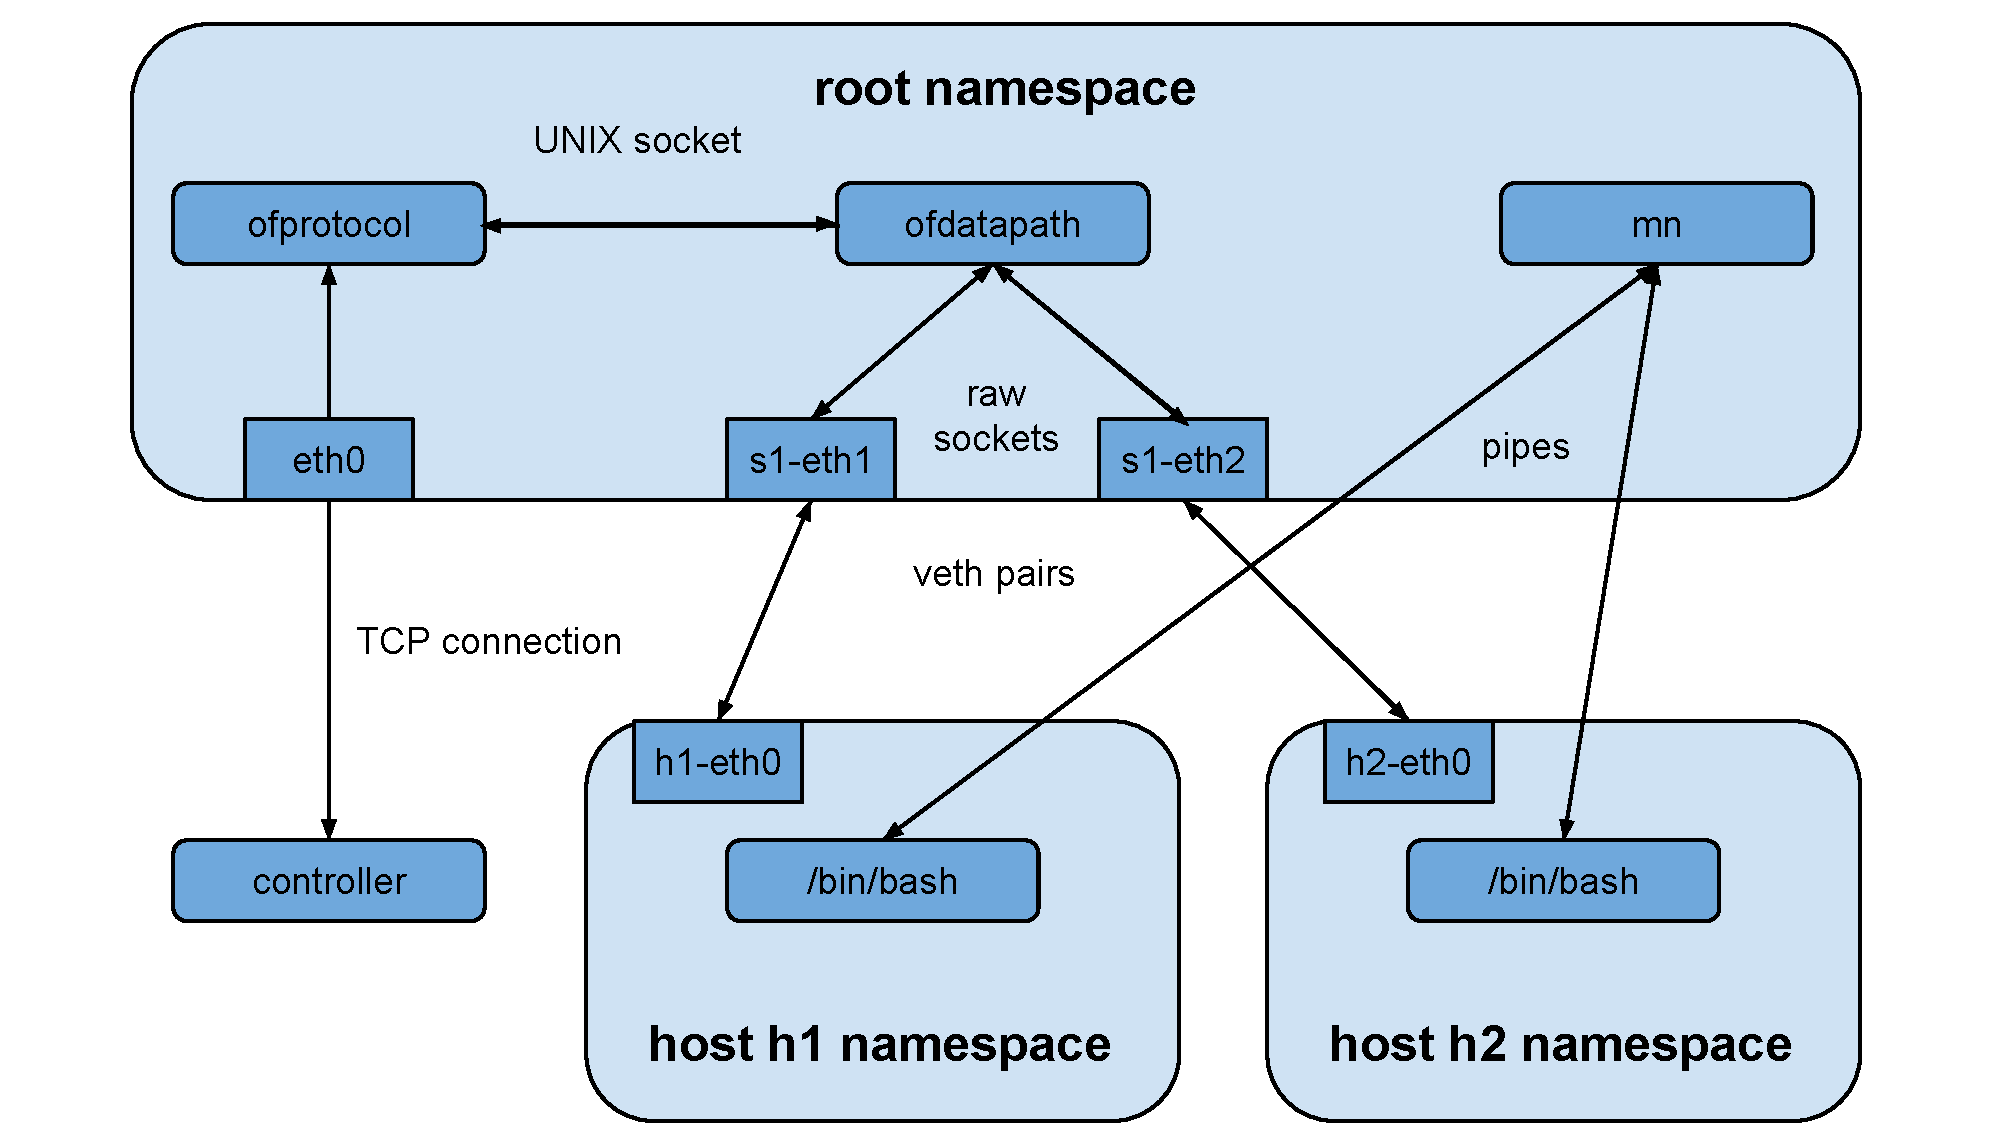
\includegraphics[width=0.85\textwidth]{img/mininet-design}
  \caption{Mininet namespaces}
  \label{fig:mininet-design}
\end{figure}

As far as flexibility goes, Mininet offers an elaborate prototyping
environment. Of all the characteristics described in \ref{sec:tcp-link},
only the TCP congestion window requires an external tool. All the other
parameters, which are Layer 2 specific, can be controlled using API calls.
Furthermore, since the API is targeted at Python, a high-level interpreted
language, topologies and simulations are easily developed.

In terms of validation of the Mininet framework as to whether it yields
relevant results or not, researchers have reproduced previous experiments
\cite{mininet-reproduce}. Not only were they able to recreate prior research
done with hardware testbeds, but thanks to the ease which Mininet simulations
can be reconfigured, they also managed to obtain extra results in some cases.

Considering the above-mentioned arguments, Mininet is undoubtedly an adequate
solution to model our tests. The testbed consists of a virtual machine running
Ubuntu 13.10 64-bit with a kernel supporting MPTCP and providing Mininet.
Using this setup, we define a simple topology using 2 hosts and 2 switches, as
seen in Figure \ref{fig:mininet-topo}. We then run iperf between the two hosts
while using different values for the link characteristics.

\begin{figure}
  \centering
  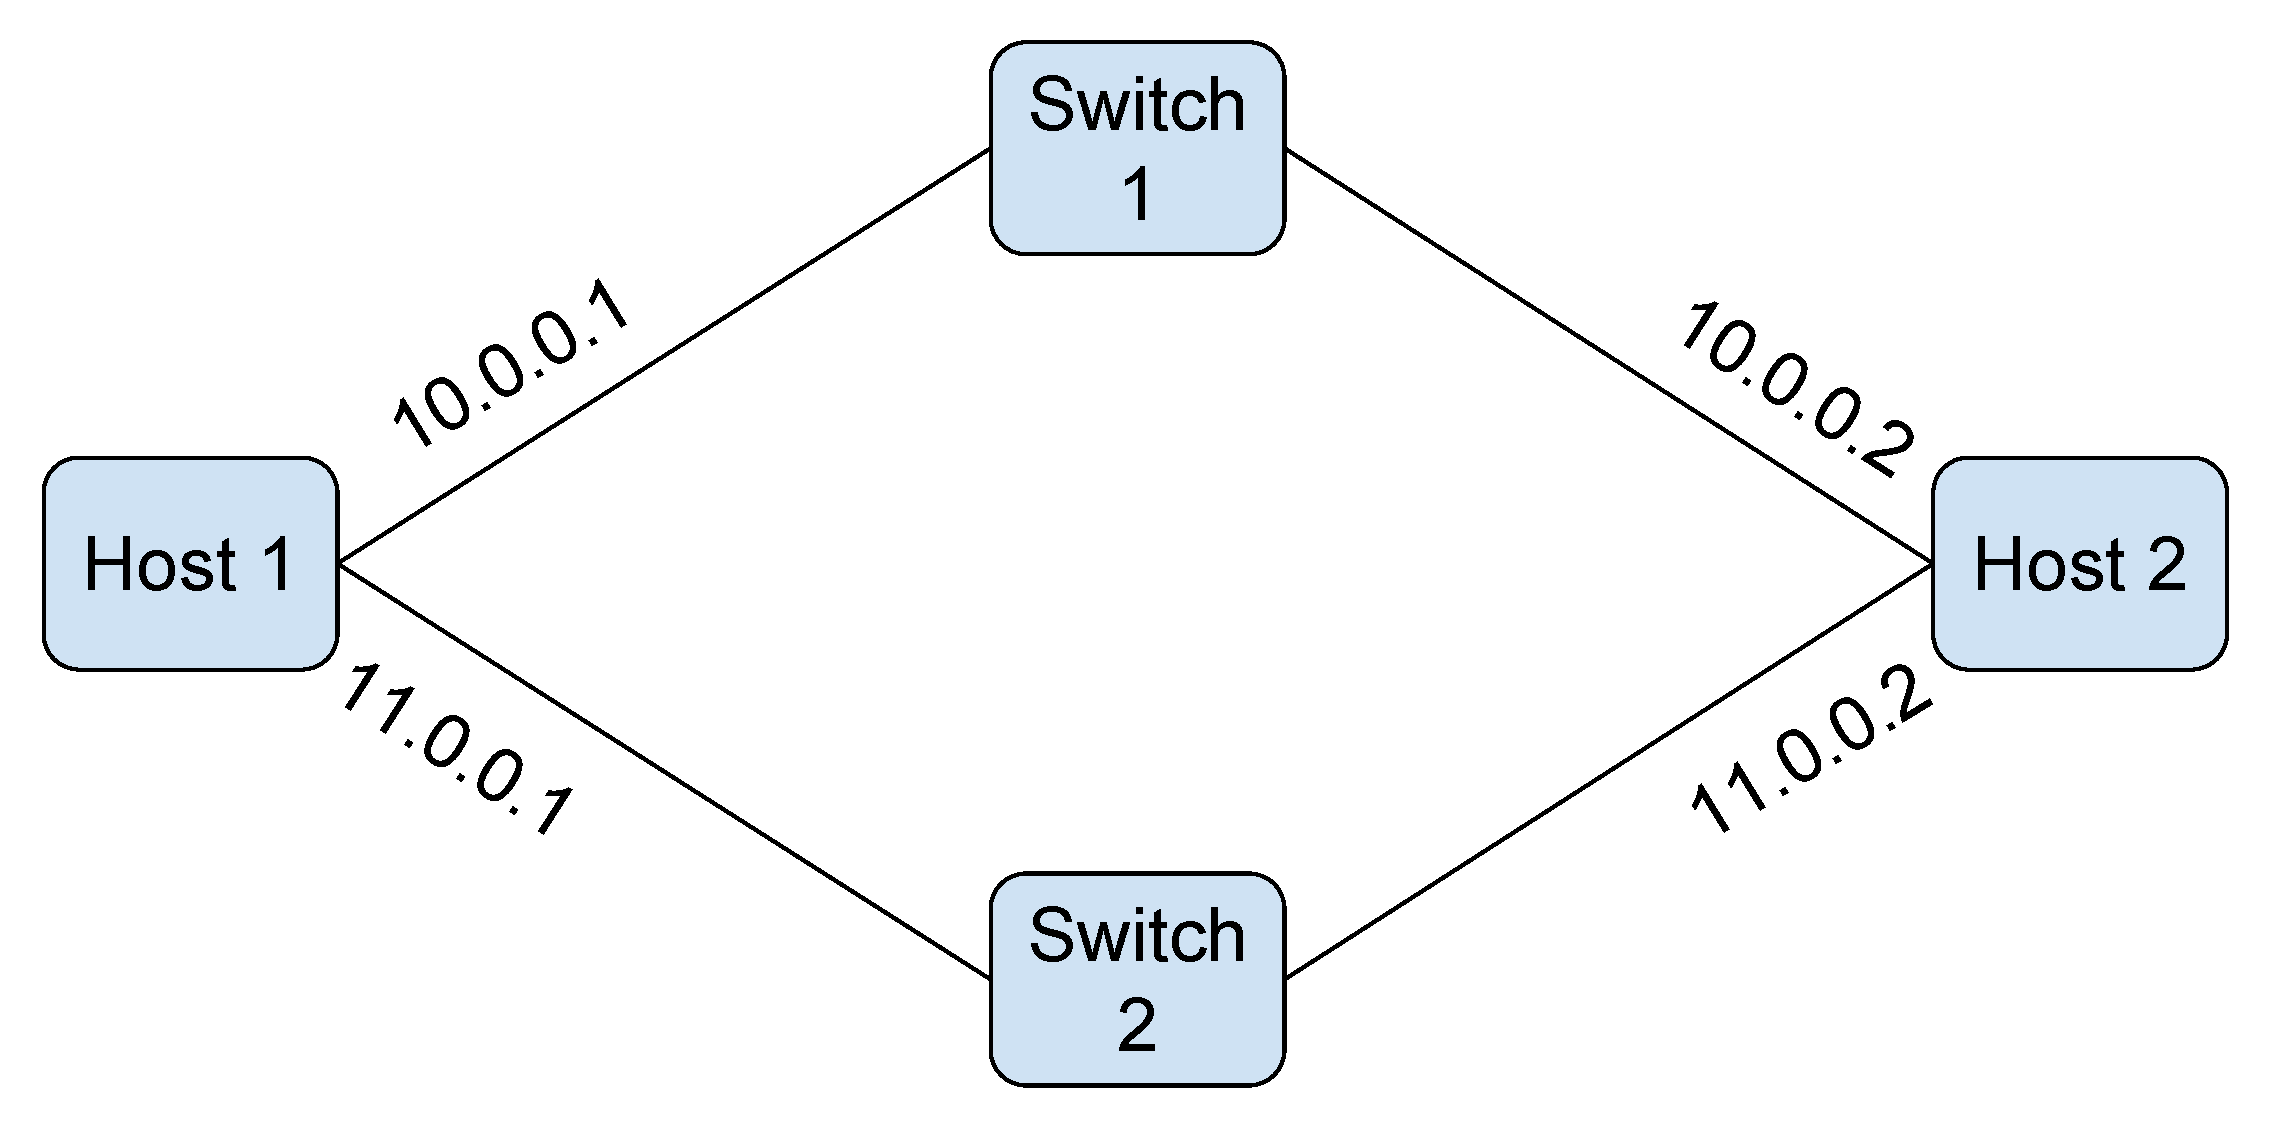
\includegraphics[width=0.5\textwidth]{img/mininet-topo}
  \caption{Mininet test topology}
  \label{fig:mininet-topo}
\end{figure}



\section{Scenarios and Results}
\label{sec:results}
% vim: set tw=78 sts=2 sw=2 ts=8 aw et ai:

We cannot properly establish the benefits of MPTCP without measuring the
achievable throughput using a single tunnel. Figures \ref{fig:udp} and
\ref{fig:tcp} show the results for a UDP tunnel and a TCP tunnel,
respectively.

\begin{figure}
  \centering
  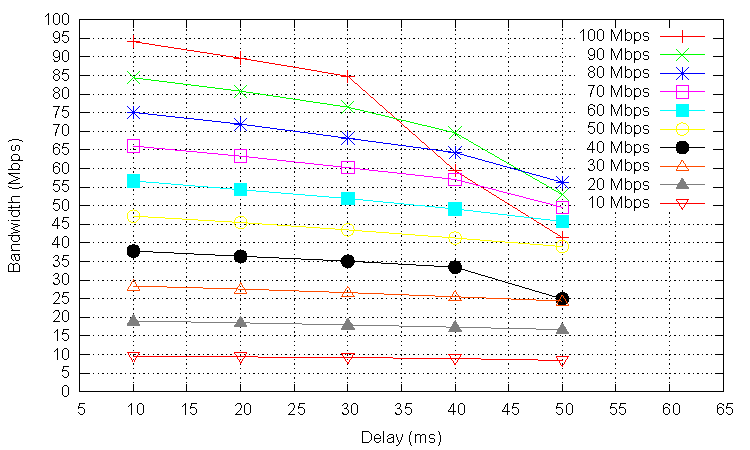
\includegraphics[width=\textwidth]{img/test-udp}
  \caption{UDP tunnel throughput}
  \label{fig:udp}
\end{figure}

\begin{figure}
  \centering
  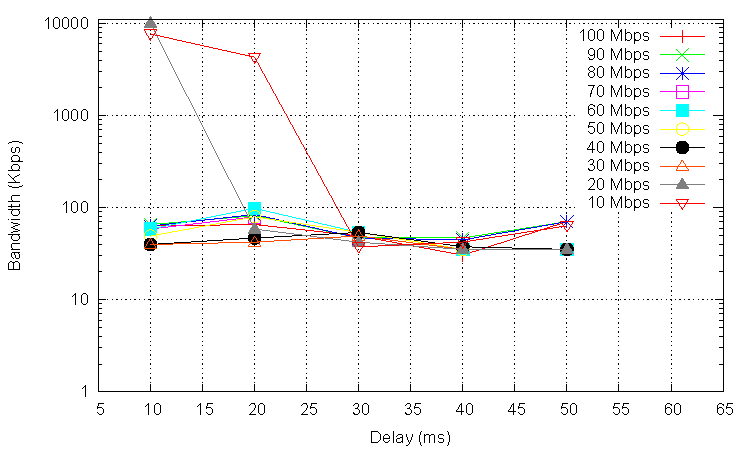
\includegraphics[width=\textwidth]{img/test-tcp}
  \caption{TCP tunnel throughput}
  \label{fig:tcp}
\end{figure}

In the case of the UDP tunnel, we notice that for lower link capacities, the
UDP tunnel manages to offer throughput close to the maximum achievable values.
That does not apply for larger bandwidths and delay. We consider that the root
cause for this is the overhead introduced by copying the data from the tunnel
device in user-space, in the OpenVPN process, and then back to kernel-space to
be sent via the Ethernet device.

The TCP tunnel exhibits poor results. Most throughput values are in the range
of 30 - 70 Kbps, with a few exceptional cases where we reach throughput up to
10 Mbps. This nondeterministic and unsatisfactory result can be explained by
taking into account the nature of our testbed. Not only are we copying large
amounts of data between user-space and kernel-space, in a virtualized
environment, but we are also attempting to run TCP traffic over a TCP tunnel.
By default, the Linux kernel uses the CUBIC congestion control algorithm with
regards to TCP connections. While this implementation has proven to be
efficient, the fact that we are encapsulating TCP traffic in TCP means that
the two instances of CUBIC will conflict with each other. We believe these are the
factors that lead to such poor performance.

Having set the baseline for what can be done using a single tunnel, we have
also conducted tests using two tunnels, using MPTCP. We have configured MPTCP
to make use of the OLIA congestion control algorithm with the goal of
observing how traffic is shifted to less congested paths, in our case the UDP
tunnel, despite the initial connection being made over the congested path, in
our case the TCP tunnel. A relevant factor in assisting MPTCP was configuring
the buffer size for a connection. We have based our tests in this regard while
taking into account the bandwidth-delay product of the link.

\begin{figure}
  \centering
  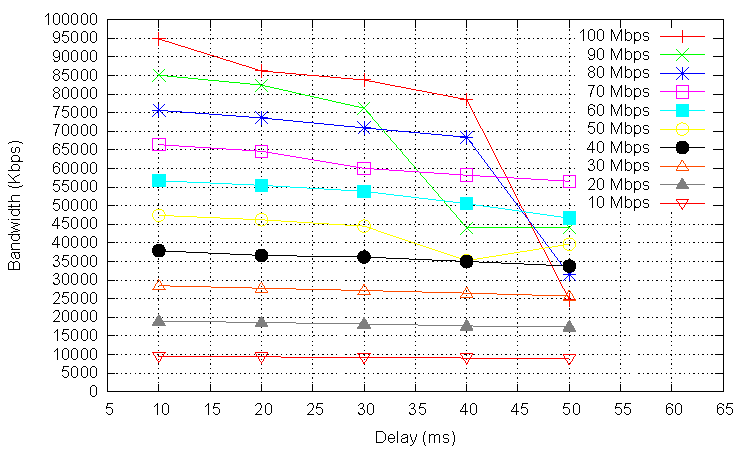
\includegraphics[width=\textwidth]{img/test-mptcp-05}
  \caption{UDP and TCP tunnels throughput, $buffer size = 0.5 \times BDP$}
  \label{fig:mptcp-0.5}
\end{figure}

\begin{figure}
  \centering
  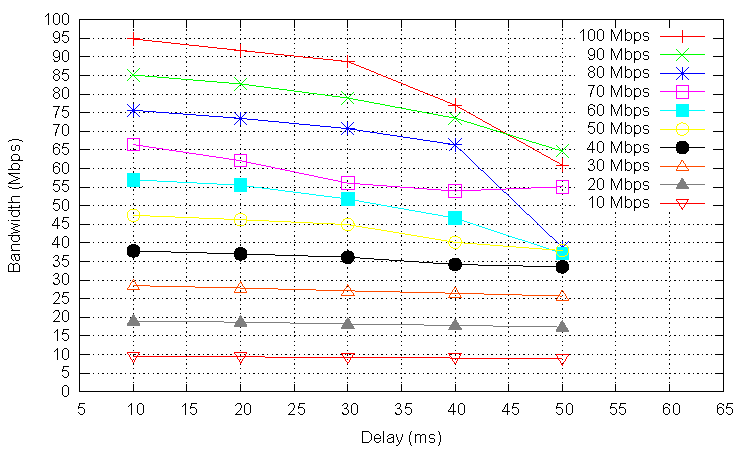
\includegraphics[width=\textwidth]{img/test-mptcp}
  \caption{UDP and TCP tunnels throughput, $buffer size = BDP$}
  \label{fig:mptcp}
\end{figure}

Figures \ref{fig:mptcp-0.5} and \ref{fig:mptcp} show the throughput when the
buffer size was either half or equal to the bandwidth-delay product. In most
cases, the results are similar or better when compared to single UDP and
single TCP. However, towards the end of the spectrum, that is for high
bandwidths and high delays, the throughput is less than that of a single UDP
tunnel, with the problem being more obvious when the buffer size is half of
the BDP. The cause lies in the fact that the buffer is insufficient and cannot
hold all the necessary packets.

\begin{figure}
  \centering
  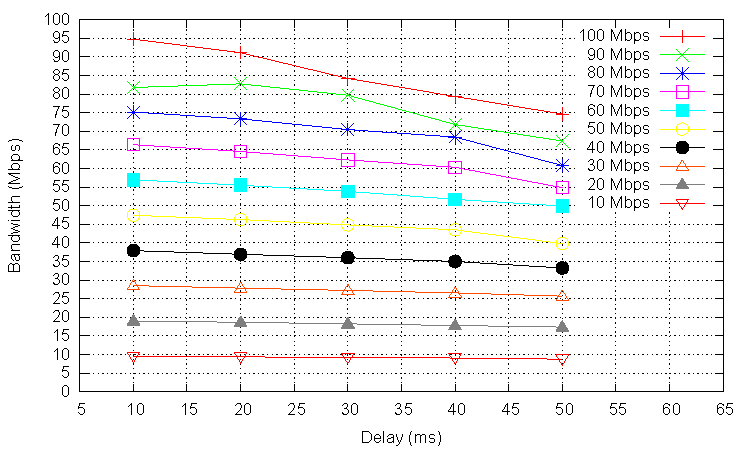
\includegraphics[width=\textwidth]{img/test-mptcp-2}
  \caption{UDP and TCP tunnels throughput, $buffer size = 2 \times BDP$}
  \label{fig:mptcp-2}
\end{figure}

Figure \ref{fig:mptcp-2} presents the throughput when the buffer size is twice
the BDP. Using this configuration, we notice that even at the high end of the
test spectrum, the results are better than single UDP or single TCP, as well
as the two previous tests. We still are not able to fully make use of the link
capacity, but we attribute this drawback to reasons mentioned above, namely
virtualization and copying of data.

While attempting to maximize link usage, we have also tested with buffer sizes
which are three times and four times the bandwidth-delay product. Figures
\ref{fig:mptcp-3} and \ref{fig:mptcp-4} summarize our results. While the lower
spectrum is comparable to previous tests, beyond an available capacity of 60 Mbps
and a delay of 30ms we notice a drop in throughput, with an even greater drop
in performance in the case of four times the BDP. This is a consequence of
granting too much memory for network buffers.

\begin{figure}
  \centering
  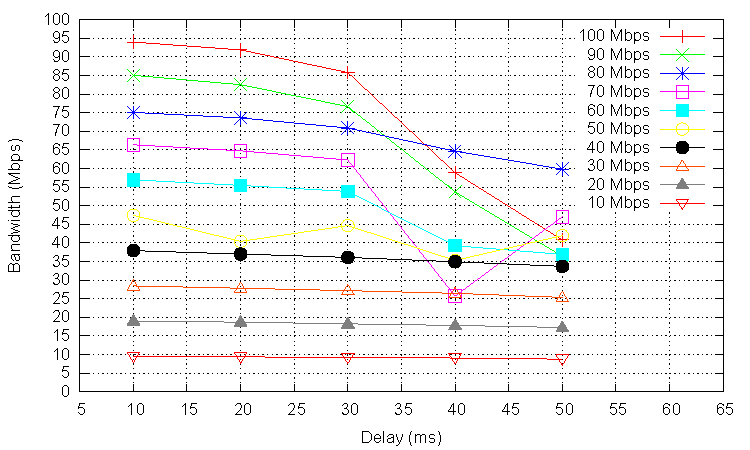
\includegraphics[width=\textwidth]{img/test-mptcp-3}
  \caption{UDP and TCP tunnels throughput, $buffer size = 3 \times BDP$}
  \label{fig:mptcp-3}
\end{figure}

\begin{figure}
  \centering
  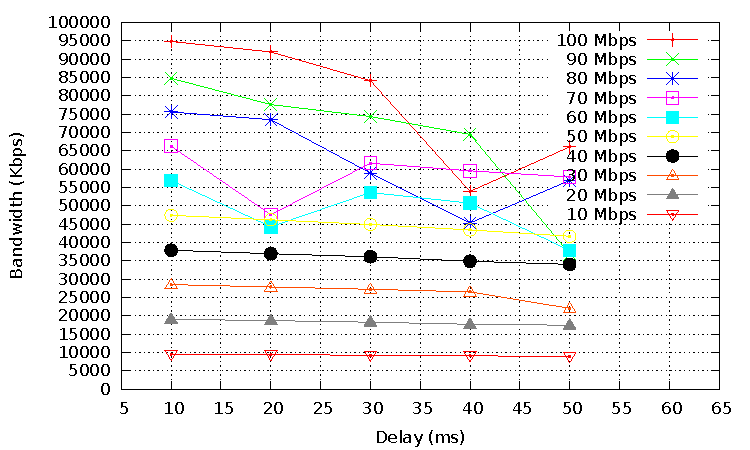
\includegraphics[width=\textwidth]{img/test-mptcp-4}
  \caption{UDP and TCP tunnels throughput, $buffer size = 4 \times BDP$}
  \label{fig:mptcp-4}
\end{figure}

\begin{figure}
  \centering
  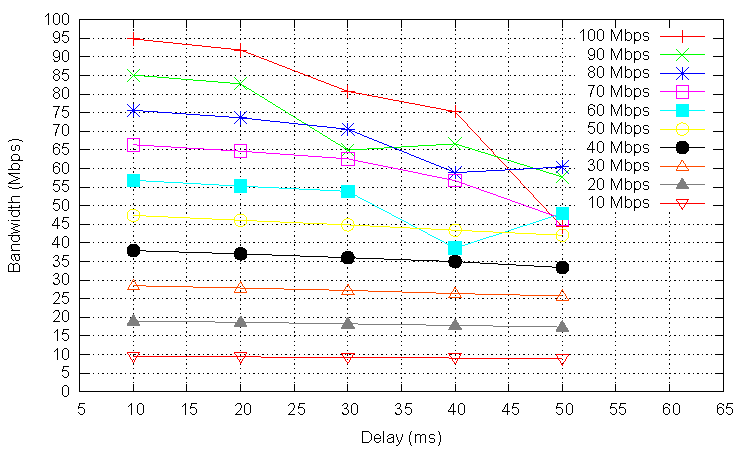
\includegraphics[width=\textwidth]{img/test-mptcp-2-crypto}
  \caption{UDP and TCP tunnels throughput, $buffer size = 2 \times BDP$, Blowfish CBC and SHA1}
  \label{fig:mptcp-2-crypto}
\end{figure}

Since our tests indicate that a buffer size twice the bandwidth-delay product
yields the best results, we have also looked at how OpenVPN's normal mode of
operation influences throughput. By default, OpenVPN uses Blowfish in CBC mode
to encrypt the information and SHA1 as a message authentication code. The
results are outlined in Figure \ref{fig:mptcp-2-crypto}. Some irregularities can be
noticed, but we attribute those to the fact that this test incurs additional
overhead due to the increased computation inherent to encryption.



\section{Conclusion and Further Work}
\label{sec:conclusion}
% vim: set tw=78 sts=2 sw=2 ts=8 aw et ai:

The current paper has looked as a prototype solution aimed at maximizing
throughput in constrained environments, based on MPTCP and OpenVPN. We have
looked at mobile networks, since carriers employ various means of restricting
the data that passes through their network. As seen in Section \ref{sec:setup}
MPTCP filtering, per port traffic shaping and even per application traffic
shaping are common approaches.

While testing our system in terms of traffic direction, congestion control and
tunnel combination, we have achieved performance on par with normal
communication, with the added benefit of encryption, multiple paths and
circumventing some operator restrictions. We have noticed that most of our
traffic is shifted onto the UDP and DNS tunnels, which is expected given the
unfavorable interaction that can arise between TCP and MPTCP congestion
control. Additionally, we have noticed aggresive filtering of the HTTP tunnel,
hinting at deep packet inspection on the side of the carrier.

We have also looked in depth at the shaping done by the operator on DNS
tunnels. To this end, we have compared our solution with and existing DNS
tunneling solution, Iodine. The results show that the mobile operator also
does deep packet inspection on DNS packets, since Iodine places tunnel data in
the DNS payload, thus achieving improved throughput.

Although there are some issues due to carriers performing deep packet
inspection on popular ports, our prototype is a feasible solution for
enhancing application throughput and bypassing firewall restrictions. Further
research could focus on encapsulating the tunnel data in the application
payload specific to the port used, thus thwarting deep packet inspection.
Another possible improvement is the usage of dynamic tunnels, where the paths
used are not established beforehand, but created and teared down as network
conditions change.


\section*{Acknowledgment}
\label{sec:acknowledgment}

The authors would like to thank XYZ for their support and dedication.

\bibliographystyle{abbrv}
\bibliography{my-report}

\end{document}
